

\section{JavaScript}

\subsection{JS-Grundlagen}
\begin{code}{Web-Konsole}
    In JS mit dem Keyword \texttt{console}:
    \begin{itemize}
        \item \texttt{console.log(message)}: Loggt eine Nachricht
        \item \texttt{console.clear()}: Löscht die Konsole
        \item \texttt{console.trace(message)}: Stack trace ausgeben
        \item \texttt{console.error(message)}: stderr ausgeben
        \item \texttt{console.time()}: Startet einen Timer
        \item \texttt{console.timeEnd()}: Stoppt den Timer
    \end{itemize}
    Website für Konsolen-API: \url{https://nodejs.org/api/console.html}
\end{code}

\begin{definition}{Datentypen}
    
    Bekannte Datentypen wie bei Java, spezielle Datentypen:
    \begin{itemize}
        \item \texttt{undefined}: Variable wurde deklariert, aber nicht initialisiert
        \item \texttt{null}: Variable wurde deklariert und initialisiert, aber nicht belegt
        \item \texttt{Symbol}: Eindeutiger, unveränderlicher Wert
        \item \texttt{Number}: Ganze Zahlen, Fließkommazahlen, NaN, Infinity
        \begin{itemize}
            \item Infinity: $1/0$, $-1/0$
            \item NaN: $0/0$, $\sqrt{-1}$
        \end{itemize}
        \item \texttt{BigInt}: Ganze Zahlen beliebiger Größe
        \item \texttt{Object}: Sammlung von Schlüssel-Wert-Paaren
        \item \texttt{Function}: Funktionen sind Objekte
    \end{itemize}
    mit dem Keyword \texttt{typeof} kann der Datentyp zurückgegeben werden
\end{definition}

\begin{center}
    \begin{tabular}{lll}
    \hline
    typeof 12 & // & 'number' \\
    typeof(12) & // 'number' &  \\
    typeof 2 n & // & 'bigint' \\
    typeof Infinity & // 'number' &  \\
    typeof NaN & // 'number' !! &  \\
    typeof 'number' & // 'string' &  \\
    \hline
    \end{tabular}
\end{center}

\begin{concept}{Variablen Definition}
    \begin{itemize}
        \item \texttt{var}: Global oder lokal
        \item \texttt{let}: Nur lokal
        \item \texttt{const}: Konstante
    \end{itemize}
\end{concept}

\begin{definition}{Variablenbindung}
    \begin{itemize}
        \item \texttt{var}: Funktionsbindung
        \item \texttt{let}: Blockbindung
        \item \texttt{const}: Blockbindung
    \end{itemize}
    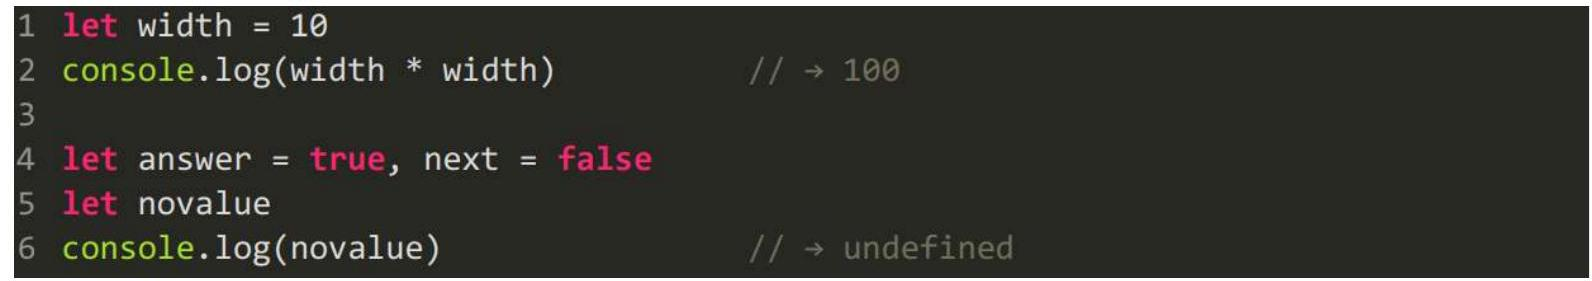
\includegraphics[width=\linewidth]{images/2024_12_29_858f09cde51177c71657g-05}
\end{definition}

\begin{definition}{Operatoren}
    \begin{itemize}
        \item Arithmetische Operatoren: $+, -, *, /, \%, ++, --$
        \item Zuweisungsoperatoren: $=, +=, -=, *=, /=, \%=, **=, <<=, >>=, >>>=, \&=, ^=, |=$
        \item Vergleichsoperatoren: $==, ===, !=, !==, >, <, >=, <=$
        \item Logische Operatoren: $\&\&, ||, !$
        \item Bitweise Operatoren: $\&, |, ^, ~, <<, >>, >>>$
        \item Sonstige Operatoren: \texttt{typeof}, \texttt{instanceof}
    \end{itemize}
\end{definition}

\begin{formula}{Vergleich mit \texttt{==} und \texttt{===}}
    \begin{itemize}
        \item \texttt{==}: Vergleicht Werte, konvertiert Datentypen
        \item \texttt{===}: Vergleicht Werte und Datentypen ohne Konvertierung
    \end{itemize}
    ebenfalls: \texttt{!=} und \texttt{!==}
\end{formula}

\begin{code}{Verzweigungen\text{,} Wiederholung und Switch Case}
    \begin{itemize}
        \item \texttt{if (condition) \{...\} else \{...\}}
        \item \texttt{switch (expression) \{ case x: ... break; default: ... \}}
        \item \texttt{for (initialization; condition; increment) \{...\}}
        \item \texttt{while (condition) \{...\}}
        \item \texttt{do \{...\} while (condition)}
        \item \texttt{for (let x of iterable) \{...\}}
    \end{itemize}
\end{code}

\begin{verbatim}
switch (<ausdruck>) {
    case <wert1>:
    break
    default:
        ...
        break
}
\end{verbatim}

\begin{verbatim}
if (<ausdruck>) \{
\} else \{
\end{verbatim}

\}

\begin{verbatim}
for (let i=1; i<50; i*=2) {
    console.log(i)
}
4 // -> 1, -> 2, -> 4, > 8, > 16, -> 32
\end{verbatim}

\begin{code}{Funktionsdefinition}
    \begin{itemize}
        \item \texttt{function name(parameters) \{...\}}
        \item \texttt{const name = (parameters) => \{...\}}
        \item \texttt{const name = parameters => \{...\}}
        \item \texttt{const name = parameters => expression}
    \end{itemize}
\end{code}

\begin{verbatim}
1 const square = function (x) {
    return x * x
}
4
5 console.log(square(12)) // -> 144
\end{verbatim}

\begin{verbatim}
1 const square1 $=(x) \Rightarrow$ \{return $x * x$ \}
2 const square2 $=x=x^{*} x$
\end{verbatim}

%\begin{example}
\begin{lstlisting}[language=JavaScript, style=base]
// Beispiel einer Funktion
function add(a, b) {
return a + b;
}
// Beispiel einer Arrow-Funktion
const add = (a, b) => a + b;
\end{lstlisting}
%\end{example}

\subsection{Objekte und Arrays}

\begin{concept}{Objekt vs Array}
    \begin{tabular}{|l|l|l|}
        \hline
        Was & Objekt & Array \\
        \hline
        Art & Attribut-Wert-Paare & Sequenz von Werten \\
        \hline
        Literalnotation & werte $=\{$ a: 1, b: 2$\}$ & liste $=[1,2,3]$ \\
        \hline
        Ohne Inhalt & werte $=\{ \}$ & liste $=[]$ \\
        \hline
        Elementzugriff & werte["a" $]$ oder werte.a & liste[0] \\
        \hline
        \end{tabular}
\end{concept}

\begin{definition}{Objekte}
    \begin{itemize}
        \item Objekt Attribute sind dynamisch und können einfach erweitert werden:
        \item Objekt Attribute können auch einfach mit dem delete keyword entfernt werden.
        \item Mit in kann überprüft werden, ob ein Attribut existiert
    \end{itemize}
\end{definition}


\begin{verbatim}
let person = {
    name: "John Baker",
    age: 23,
    "exam results": [5.5, 5.0, 5.0, 6.0, 4.5]
}
\end{verbatim}

\begin{verbatim}
    let obj = { message: "not yet implemented" }
    obj.ready = false
> obj
{ message: 'not yet implemented', ready: false }
> obj.attr
undefined
\end{verbatim}

\begin{verbatim}
> let obj = { message: "ready", ready: true, tasks: 3 }
> delete obj.message
> obj.tasks = undefined
> obj
{ ready: true, tasks: undefined }
> "message" in obj
false
> "tasks" in obj
true
\end{verbatim}

\begin{definition}{Methoden}
    Ein Objekt kann auch Methoden enthalten:
\end{definition}

\begin{verbatim}
> let cat = { type: "cat", sayHello: () => "Meow" }
> cat.sayHello
[Function: sayHello]
    > cat.sayHello()
'Meow'
\end{verbatim}

\begin{code}{Arrays}

    Verschiedene Hilfsfunktionen:

    \begin{itemize}
        \item Array.isArray()
        \item .push()
        \item .pop()
        \item Indexof, lastIndexOf
        \item Concat
        \item slice
        \item Shift, unshift
        \item .forEach(item => ....)
        \item .filter(item => .....)
        \item .map(item => ...)
    \end{itemize}

    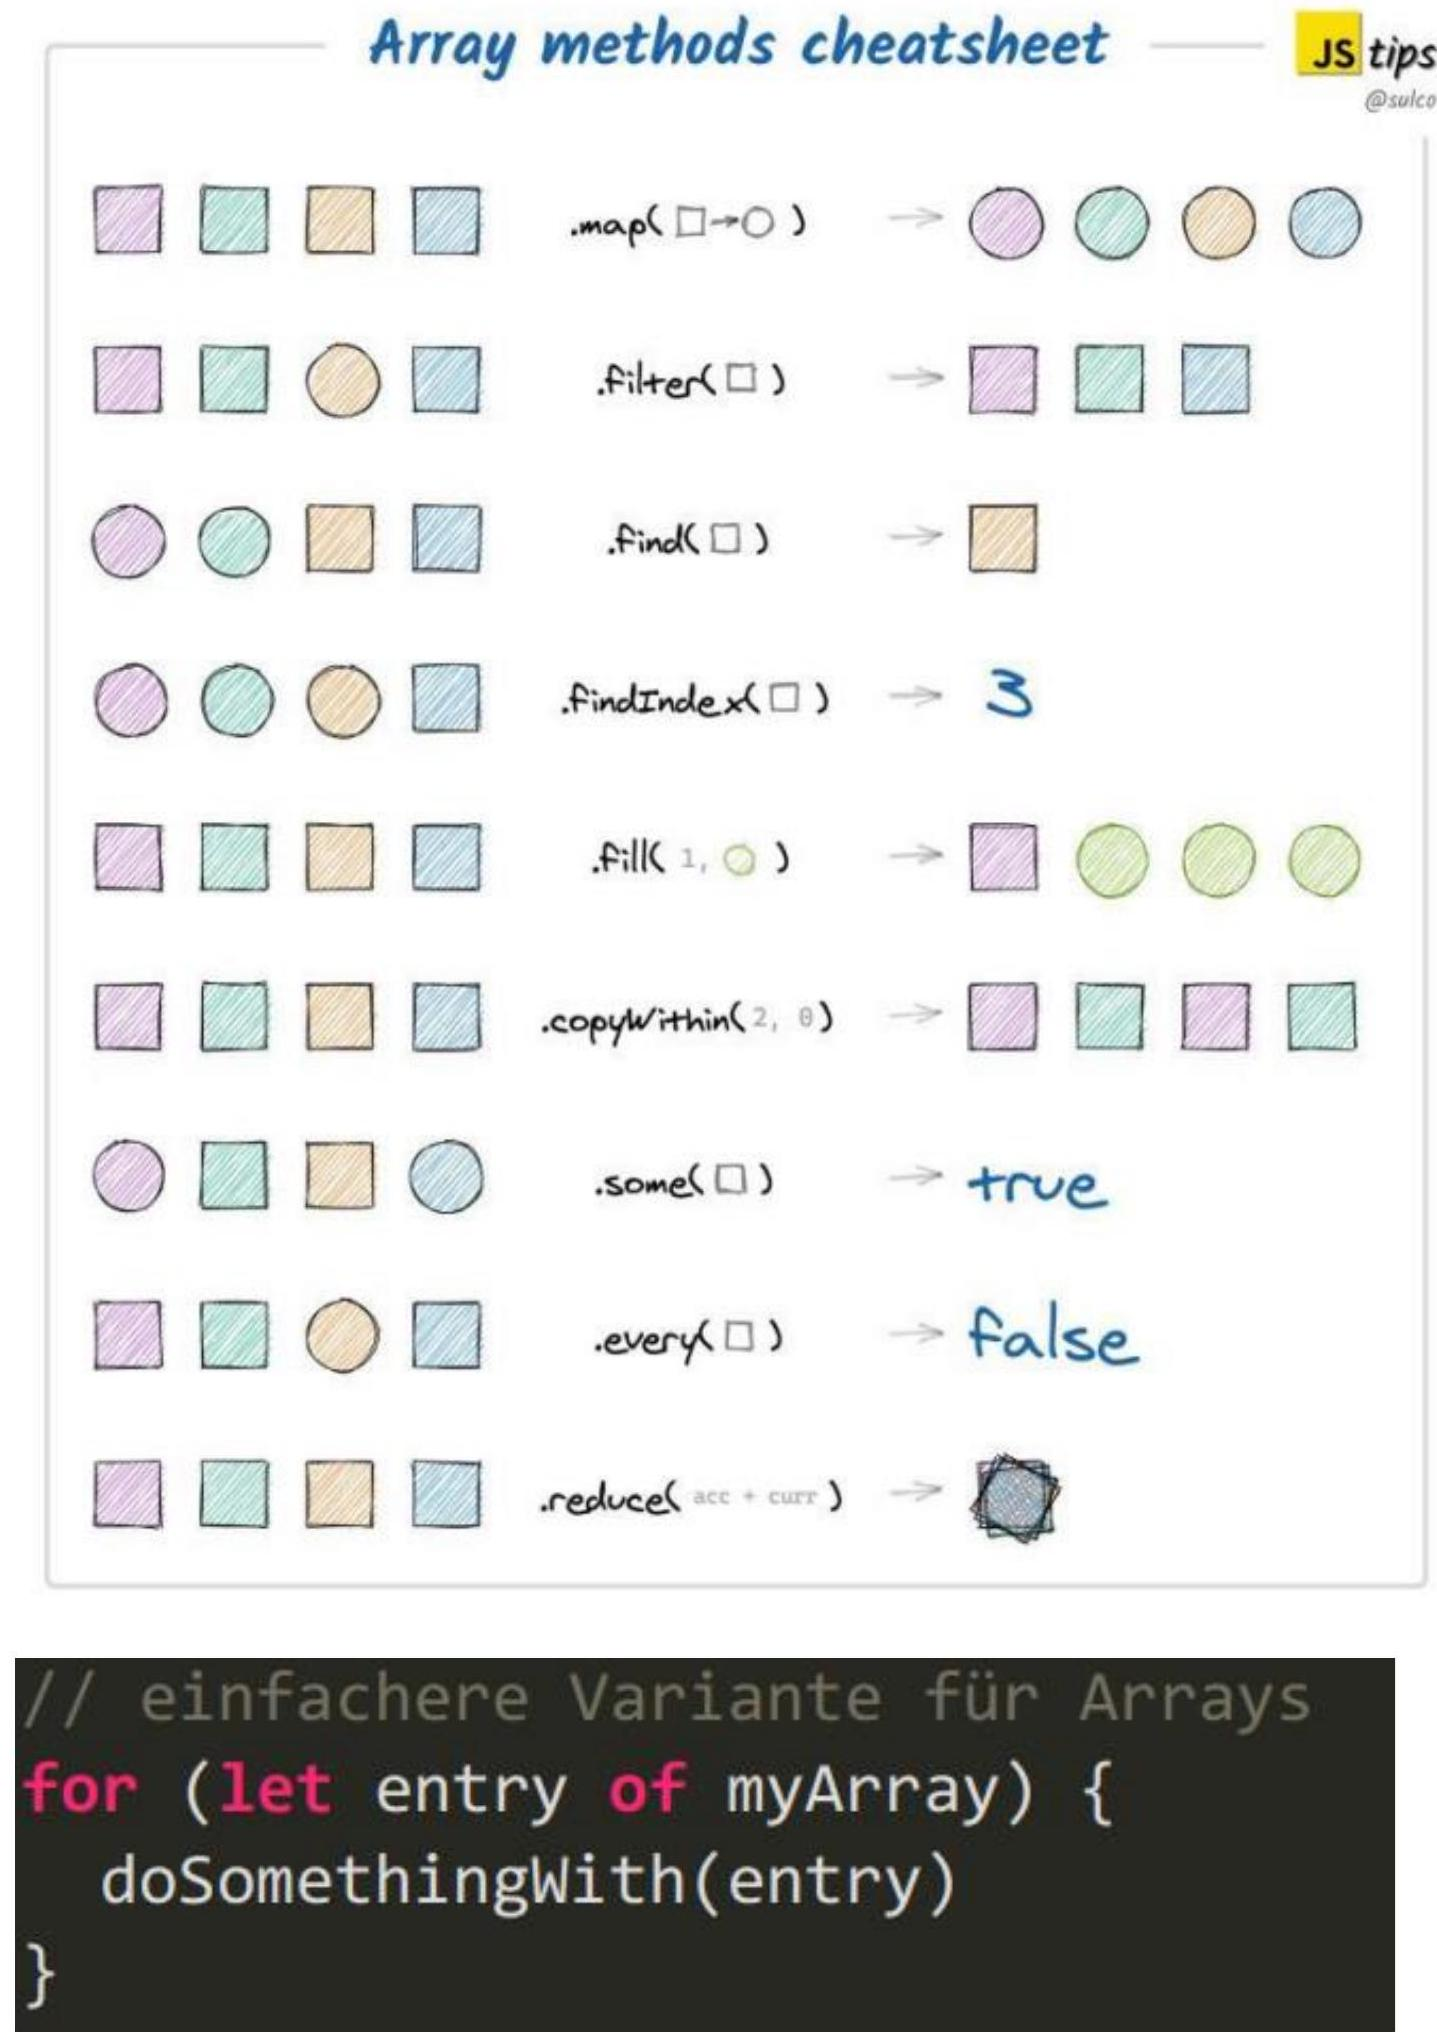
\includegraphics[width=\linewidth]{images/2024_12_29_858f09cde51177c71657g-08}
\end{code}

begin{concept}{Json: JavaScript Object Notation}
\begin{itemize}
    \item Daten-Austauschformat, nicht nur für JavaScript
    \item Orientiert an Notation für JavaScript-Objektliterale
  \end{itemize}
  https://www.json.org/json-en.html
\end{concept}
  
  \begin{verbatim}
  > JSON.stringify({ type: "cat", name: "Mimi", age: 3})
  '{"type":"cat", "name":"Mimi", "age":3}'
  > JSON.parse('{"type":"cat","name":"Mimi","age":3}')
  { type: 'cat', name: 'Mimi', age: 3 }
  \end{verbatim}


\subsection{Funktionen und funktionale Programmierung}

\begin{definition}{Funktionen}
    \begin{itemize}
        \item Funktionen sind spezielle, aufrufbare Objekte
        \item Man kann ihnen jederzeit Attribute oder Methoden hinzufügen
        \item Sie haben bereits vordefinierte Methoden
      \end{itemize}
\end{definition}

\begin{verbatim}
    const add = (x, y) => x + y
    add.doc = "This function adds two values"
        add(3,4)
    7
        add.doc
    'This function adds two values'
\end{verbatim}

\begin{concept}{Modulsystem in JavaScript}
    \begin{itemize}
        \item \texttt{import} und \texttt{export} für Module
        \item \texttt{export default} für Standardexport
        \item \texttt{import \{name\} from 'module'} für benannte Exports
        \item \texttt{import * as name from 'module'} für alle Exports
    \end{itemize}
\end{concept}

\begin{verbatim}
    1 /* car-lib.js */
    2}\mathrm{ const car = {
    3 brand: 'Ford',
    4 model: 'Fiesta'
    5 }
    6
    7 module.exports = car
    1 /* other js file */
    2 const car = require('./car-lib')
\end{verbatim}

\subsection{Prototypen von Objekten}

\begin{definition}{Prototypen}
    \begin{itemize}
        \item Die meisten Objekte haben ein Prototyp-Objekt.
        \item Dieses fungiert als Fallback für Attribute und Methoden.
      \end{itemize}
\end{definition}

\begin{verbatim}
    > Object.getPrototypeOf(Math.max) == Function.prototype
    true
    > Object.getPrototypeOf([]) == Array.prototype
    true
    > Object.getPrototypeOf(Function.prototype) == Object.prototype
    true
    > Object.getPrototypeOf(Array.prototype) == Object.prototype
    true
\end{verbatim}

\begin{code}{Prototypen-Kette}
    \begin{verbatim}
        function Employee (name, salary) {
            Person.call(this, name)
            this.salary = salary
        }
        Employee.prototype = new Person()
        Employee.prototype.constructor = Employee
        let e17 = new Employee("Mary", 7000)
        console.log(e17.toString()) /* -> Person with name 'Mary' */
        console.log(e17.salary) /* -> 7000 */
        \end{verbatim}
        
        Call, apply, bind
        
        \begin{itemize}
          \item Weitere Argumente von call : Argumente der Funktion
          \item Weiteres Argument von apply : Array mit den Argumenten
          \item Erzeugt neue Funktion mit gebundenem this
        \end{itemize}
\end{code}

\begin{code}{Klassen}
    \begin{itemize}
        \item Klassen sind syntaktischer Zucker für Prototypen
        \item Klassen können Attribute und Methoden enthalten
        \item Klassen können von anderen Klassen erben
    \end{itemize}

    \begin{verbatim}
        class Person {
            constructor (name) {
                this.name = name
            }
            toString () {
                return `Person with name '${this.name}'
            }
        }
        let p35 = new Person("John")
        console.log(p35.toString()) // -> Person with name 'John'
        \end{verbatim}
\end{code}

\begin{code}{Vererbung}
    \begin{verbatim}
        class Employee extends Person {
            constructor (name, salary) {
                super(name)
                this.salary = salary
            }
            toString () {
                return `${super.toString()} and salary ${this.salary}
            }
        }
        let e17 = new Employee("Mary", 7000);
        console.log(e17.toString()) /* -> Person with name 'Mary' and salary 7000 */
        console.log(e17.salary) /* -> 7000 */
        \end{verbatim}
\end{code}

\begin{code}{Getter und Setter}
    \begin{verbatim}
        class PartTimeEmployee extends Employee {
            constructor (name, salary, percentage) {
                super(name, salary)
                this.percentage = percentage
            }
            get salary100 () { return this.salary * 100 / this.percentage}
            set salary100 (amount) { this.salary = amount * this.percentage / 100 }
        }
        let e18 = new PartTimeEmployee("Bob", 4000, 50)
        console.log(e18.salary100) /* -> 8000 */
        e18.salary100 = 9000
        console.log(e18.salary) /* \ 4500 */
        \end{verbatim}
\end{code}

\subsection{Asynchrone Programmierung}

\begin{definition}{File API}
    Mit require('fs') wird auf die File-Api zugegriffen.
\end{definition}

\section*{Datei-Informationen}
\begin{verbatim}
const fs = require('fs')
fs.stat('test.txt' , (err, stats) => {
    if (err) {
    console.error(err)
    return
    }
    stats.isFile() /* true */
    stats.isDirectory() /* false */
    stats.isSymbolicLink() /* false */
stats.size /* 1024000 = ca 1MB */
})
\end{verbatim}

\section*{Pfade der Datei}
Um Pfad-informationen einer Datei zu ermitteln muss man dies mit require('path') machen.

\begin{verbatim}
const path = require('path')
const notes = '/users/bkrt/notes.txt'
path.dirname(notes) /* /users/bkrt */
path.basename(notes) /* notes.txt */
path.extname(notes) /* .txt */
path.basename(notes, path.extname(notes)) /* notes */
\end{verbatim}

\section*{Lesen aus einer Datei}
\begin{verbatim}
const fs = require('fs')
fs.readFile('/etc/hosts',"utf8", (err, data) => {
        if (err) throw err
        console.log(data)
})
\end{verbatim}

\section*{Dateien schreiben}
\begin{verbatim}
1 const fs = require('fs')
2}\mathrm{ const content = 'Node was here!'
3 fs.writeFile('/Users/bkrt/test.txt', content, (err) => {
4 if (err) {
5 console.error(`Failed to write file: ${err}`)
6 return
7 }
8 ** file written successfully */
9 })
\end{verbatim}

Weitere FS Funktionen

\begin{center}
\begin{tabular}{|l|l|}
\hline
Funktion & Bezeichnung \\
\hline
fs.access & Zugriff auf Datei oder Ordner prüfen \\
\hline
fs.mkdir & Verzeichnis anlegen \\
\hline
fs.readdir & Verzeichnis lesen, liefert Array von Einträgen \\
\hline
fs.rename & Verzeichnis umbenennen \\
\hline
fs.rmdir & Verzeichnis löschen \\
\hline
fs.chmod & Berechtigungen ändern \\
\hline
fs.chown & Besitzer und Gruppe ändern \\
\hline
fs.copyFile & Datei kopieren \\
\hline
fs.link & Besitzer und Gruppe ändern \\
\hline
fs.symlink & Symbolic Link anlegen \\
\hline
fs.watchFile & Datei auf Änderungen überwachen \\
\hline
\end{tabular}
\end{center}

\section*{Callbacks}
Ein Callback ist eine Funktion, welche als Argument einer anderen Funktion übergeben wird und erst aufgerufen wird, wenn das Ereignis eingetreten ist. In der folgenden Abbildung wird die KlickFunktion vom Button mit der Id «Button» abonniert.

1 document.getElementById('button').addEventListener('click', () => \{\\
2 //item clicked\\
3 \})

\section*{SetTimeout}
\begin{itemize}
  \item Mit setTimeout kann Code definiert werden, der zu einem späteren Zeitpunkt ausgeführt werden soll
  \item Eintrag in die Timer-Liste, auch wenn Zeit auf 0 gesetzt wird
  \item Kann mit clearTimeout entfernt werden
\end{itemize}

1 setTimeout(() => \{\\
2 /* runs after 50 milliseconds */\\
3 \}, 50)

\section*{SetInterval}
\begin{itemize}
  \item Callback alle n Millisekunden in die Callback Queue eingefügt
  \item Kann mit clearInterval beendet werden
\end{itemize}

\begin{verbatim}
1 const id = setInterval(() => {
2 // runs every 2 seconds
3 }, 2000)
4 clearInterval(id)
\end{verbatim}

\section*{SetImmediate}
\begin{verbatim}
1 setImmediate(() => {
2 console.log('immediate')
3 })
4
\end{verbatim}

\section*{Event-Modul (EventMitter)}
\begin{itemize}
  \item EventEmitter verwaltet Liste von Listeners zu bestimmten Events
  \item Listener für das Event können hinzugefügt oder entfernt werden
  \item Event kann ausgelöst werden $\rightarrow$ Listener werden informiert
\end{itemize}

\section*{Listener hinzufügen}
\begin{verbatim}
4 const EventEmitter = require('events')
5 const door = new EventEmitter()
6
7 door.on('open', () => \{
8 console.log('Door was opened')
9 \})
\end{verbatim}

\section*{Event auslösen}
\begin{verbatim}
1 door.on('open', (speed) => \{
2 console.log(`Door was opened, speed: \$\{speed /| 'unknown'\}`)
3 \})
4
5 door.emit('open')
6 door.emit('open', 'slow')
\end{verbatim}

\section*{Promises}
Ist ein Platzhalter für einen Wert, der erst später voraussichtlich verfügbar sein wird.

\begin{verbatim}
Funktion mit Promise
\end{verbatim}

\begin{verbatim}
function readFilePromise (file) {
\end{verbatim}

function readFilePromise (file) \{\\
let promise = new Promise(\\
let promise = new Promise(\\
function resolver (resolve, reject) \{\\
function resolver (resolve, reject) \{\\
fs.readFile(file, "utf8", (err, data) => \{\\
fs.readFile(file, "utf8", (err, data) => \{\\
if (err) reject(err)\\
if (err) reject(err)\\
else resolve(data)\\
else resolve(data)\\
\})\\
\})\\
\})\\
\})\\
return promise\\
return promise\\
\}

\begin{verbatim}
}
\end{verbatim}

Gibt nun ein Promise-Object zurück

\section*{Promise-Konstruktor erhlt resolver-Funktion}
Rückgabe einer Promise: potentieller Wert kann später erfüllt oder zurückgewiesen werden

\begin{itemize}
  \item Rückgabe einer Promise: potentieller Wert
  \item kann später erfüllt oder zurückgewiesen werden
\end{itemize}

Aufruf neu:

\begin{verbatim}
readFilePromise('/etc/hosts')
    .then(console.log)
    .catch(() => {
        console.log("Error reading file")
    })
\end{verbatim}

\section*{Promise-Zustände}
\begin{itemize}
  \item pending: Ausgangzustand
  \item fulfilled: erfolgreich abgeschlossen
  \item rejected: ohne Erfolg abgeschlossen
  \item Nur ein Zustandsübergang möglich
  \item Zustand in Promise-Objekt gekapselt\\
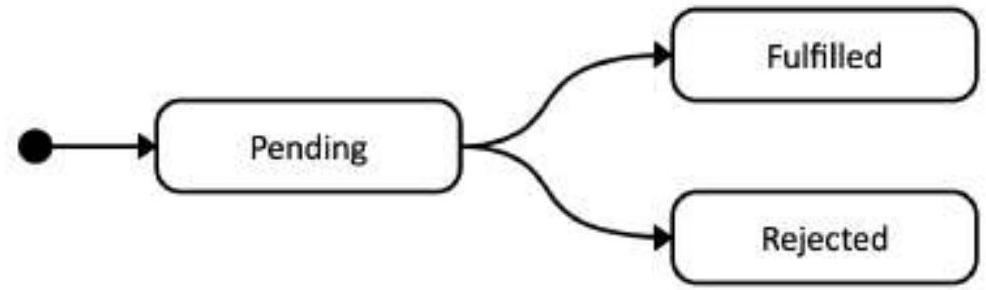
\includegraphics[max width=\textwidth, center]{2024_12_29_858f09cde51177c71657g-14}
\end{itemize}

\section*{Promises Verknüpfen}
\begin{itemize}
  \item Then-Aufruf gibt selbst Promise zurück
  \item Catch-Aufruf ebenfalls, per Default erfüllt
  \item So können diese Aufrufe verkettet werden
  \item Promise, welche unmittelbar resolved wird: Promise.resolve (...)
  \item Promise, welche unmittelbar rejected wird: Promise.reject (...)
\end{itemize}

\section*{Promise.all()}
\begin{itemize}
  \item Erhält Array von Promises
  \item Erfüllt mit Array der Result, wenn alle erfüllt sind
  \item Zurückgewiesen sobald eine Promise zurückgewiesen wird
\end{itemize}

\section*{Promise.race()}
\begin{itemize}
  \item Erhält Array von Promises
  \item Erfüllt sobald eine davon erfüllt ist
  \item Zurückgewiesen sobald eine davon zurückgewiesen wird
\end{itemize}

\section*{ASYNC/AWAIT}
Beispiel 1

\begin{verbatim}
/* Bekanntes Beispiel */
const readHosts =() => {
    readFilePromise('/etc/hosts')
        .then(console.log)
        . catch(() => {
            console.log("Error reading file")
        })
}
/* Mit async/await */
const readHosts = async () => {
    try {
        console.log(await readFilePromise('/etc/hosts'))
    }
    catch (err) {
        console.log("Error reading file")
    }
}
\end{verbatim}

\section*{Beispiel 2}
\begin{verbatim}
function resolveAfter2Seconds (x) {
    return new Promise(resolve => {
        setTimeout(() => {
            resolve(x)
        }, 2000)
    })
}
async function add1(x) {
    var a = resolveAfter2Seconds(20)
    var b = resolveAfter2Seconds(30)
    return x + await a + await b
}
add1(10).then(console.log)
\end{verbatim}

\subsection{Webserver}
Die Standard-Ports von einem Webserver sind 80 und 443. Der Webserver wartet auf eine Anfrage vom Client.

\section*{Server im Internet}
\begin{itemize}
  \item Wartet auf Anfragen auf bestimmtem Port
  \item Client stellt Verbindung her und sendet Anfrage
  \item Server beantwortet Anfrage
\end{itemize}

\begin{center}
\begin{tabular}{|l|l|}
\hline
Port & Service \\
\hline
$\mathbf{2 0}$ & FTP - Data \\
\hline
$\mathbf{2 1}$ & FTP - Control \\
\hline
$\mathbf{2 2}$ & SSH Remote Login Protocol \\
\hline
$\mathbf{2 3}$ & Telnet \\
\hline
$\mathbf{2 5}$ & Simple Mail Transfer Protocol (SMTP) \\
\hline
$\mathbf{5 3}$ & Domain Name System (DNS) \\
\hline
$\mathbf{8 0}$ & HTTP \\
\hline
$\mathbf{4 4 3}$ & HTTPs \\
\hline
\end{tabular}
\end{center}

File-Transfer (File Server)\\
Um Dateien auf einem File-Server auszutauschen, werden die Protokolle FTP (File Transfer Protocol) und SFTP (SSH File Transfer Protocol) verwendet.

HTTP\\
HTTP-Requests

\begin{center}
\begin{tabular}{|l|l|}
\hline
Methode & Beschreibung \\
\hline
GET & Ressource laden \\
\hline
POST & Information senden \\
\hline
PUT & Ressource anlegen, überschreiben \\
\hline
PATCH & Ressource anpassen \\
\hline
DELETE & Ressource löschen \\
\hline
\end{tabular}
\end{center}

HTTP-Response Codes

\begin{center}
\begin{tabular}{|l|l|}
\hline
Code & Beschreibung \\
\hline
$\mathbf{1 x x}$ & Information (101 Switching protocols) \\
\hline
$\mathbf{2 x x}$ & Erfolg (200 OK) \\
\hline
$\mathbf{3 x x}$ & Weiterleitung (301 Moved permanently) \\
\hline
$\mathbf{4 x x}$ & Fehler in Anfrage (403 Forbidden, 404 Not Found) \\
\hline
$\mathbf{5 x x}$ & Server-Fehler (501 Not implemented) \\
\hline
\end{tabular}
\end{center}

Node.js Webserver\\
Einfacher Webserver

\begin{verbatim}
const {createServer} = require("http")
Let server = createServer((request, response) => {
    response.writeHead(200, {"Content-Type": "text/html"})
    response.write(`
        <h1>Hello!</h1>
        <p>You asked for <code>${request.url}</code></p>`)
    response.end()
})
server.listen(8000)
console.log("Listening! (port 8000)")|
\end{verbatim}

\section*{Einfacher Webclient}
\begin{verbatim}
onst {request} = require("http")
let requestStream = request({
    hostname: "eloquentjavascript.net",
        path: "/20_node.html",
        method: "GET"
        headers: {Accept: "text/html"}
}, response => {
        console.log("Server responded with status code", response.statusCode)
})
requestStream.end()
\end{verbatim}

\section*{Server und Client mit Streams}
\begin{verbatim}
const {createServer} = require("http")
createServer((request, response) => {
    response.writeHead(200, {"Content-Type": "text/plain"})
        request.on("data", chunk =>
            response.write(chunk.toString().toUpperCase()))
        request.on("end" , () => response.end())
    }).listen(8000)
\end{verbatim}

\begin{verbatim}
const \{request\} = require("http")
Let $\mathrm{rq}=$ request(\{
    hostname: "localhost",
    port: 8000,
    method: "POST"
\}, response => \{
    response.on("data", chunk =>
    process.stdout.write(chunk.toString()));
\})
rq.write("Hello server\n")
rq.write("And good bye\n")
rq.end()
\end{verbatim}

\section*{REST API}
\begin{itemize}
  \item REST: Representational State Transfer
  \item Zugriff auf Ressourcen über ihre Adresse (URI)
  \item Kein Zustand: jede Anfrage komplett unabhängig
  \item Kein Bezug zu vorhergehenden Anfragen
  \item Alle nötigen Informationen in Anfrage enthalten
  \item Verwenden der HTTP-Methoden: GET , PUT , POST , ...\\
(WBE\_Alles.pdf) Page 363.\\
Express.js\\
Express.Js ist ein minimales, aber flexibles Framework für Web-apps. Es hat zahlreiche Utilities und Erweiterungen. Express.js basiert auf Node.js.
\end{itemize}

\section*{http://expressjs.com}
\section*{Installation}
\begin{itemize}
  \item Der Schritt npm init fragt eine Reihe von Informationen (Projektname, Version, ...) zum Projekt ab
  \item Als Entry Point ist hier index.js voreingestellt
  \item Das kann zum Beispiel in app.js geändert werden.
\end{itemize}

\begin{verbatim}
$ mkdir myapp
$ cd myapp
$ npm init
$ npm install express --save
\end{verbatim}

\section*{Beispiel: Express Server}
\begin{verbatim}
const express = require('express')
const app = express()
const port = 3000
app.get('/', (req, res) => {
        res.send('Hello World!')
})
app.listen(port, () => {
    console.log(`Example app listening at http://localhost:${port}`)
}})
\end{verbatim}

\begin{verbatim}
Routing
\end{verbatim}

\begin{verbatim}
app.get('/', function (req, res) {
\end{verbatim}

app.get('/', function (req, res) \{\\
res.send('Hello World!')\\
res.send('Hello World!')\\
\})\\
\})\\
app.post('/', function (req, res) \{\\
app.post('/', function (req, res) \{\\
res.send('Got a POST request')\\
res.send('Got a POST request')\\
\})\\
\})\\
app.put('/user', function (req, res) \{\\
app.put('/user', function (req, res) \{\\
res.send('Got a PUT request at /user')\\
res.send('Got a PUT request at /user')\\
\})\\
\})\\
app.delete('/user', function (req, res) \{\\
app.delete('/user', function (req, res) \{\\
res.send('Got a DELETE request at /user')\\
res.send('Got a DELETE request at /user')\\
\})

\begin{verbatim}
})
\end{verbatim}

Jasmine (Testing)

\section*{BEISPIEL (ZUGEHÖRIGE TESTS)}
\begin{verbatim}
/* PlayerSpec.js - Auszug */
describe("when song has been paused", function() {
    beforeEach(function() {
        player.play(song)
        player.pause()
    })
    it("should indicate that the song is currently paused", function() {
        expect(player.isPlaying).toBeFalsy()
        /* demonstrates use of 'not' with a custom matcher */
        expect(player).not.toBePlaying(song)
    })
    it("should be possible to resume", function() {
        player.resume()
        expect(player.isPlaying).toBeTruthy()
        expect(player.currentlyPlayingSong).toEqual(song)
    })
})
\end{verbatim}

\section*{JASMINE: MATCHER}
\begin{verbatim}
expect([1, 2, 3]).toEqual([1, 2, 3])
expect(12).toBeTruthy()
expect("").toBeFalsy()
expect("Hello planet").not.toContain("world")
expect(null).toBeNull()
expect(8).toBeGreaterThan(5)
expect(12.34).toBeCloseTo(12.3, 1)
expect("horse_ebooks.jpg").toMatch(/\w+.(jpg|gif|png|svg)/i)
\end{verbatim}

\section*{JASMINE: TESTS DURCHFÜHREN}
\$ npx jasmine\\
Randomized with seed 03741\\
Started

5 specs, 0 failures\\
Finished in 0.014 seconds\\
Randomized with seed 03741 (jasmine --random=true --seed=03741)\\